% ============================================================
%  يُترجَم بـ XeLaTeX  (في Overleaf: Menu → Compiler → XeLaTeX)
%  الخط: Amiri (متوفر في Overleaf، أو حمّله من github.com/aliftype/amiri)
% ============================================================
\documentclass[12pt,a4paper]{article}
\usepackage[a4paper,margin=1.7cm,top=2.3cm,bottom=2.9cm,headheight=15pt,footskip=1.5cm]{geometry}
\usepackage{amsmath,amssymb}
\usepackage{icomma}
\usepackage[english,bidi=default,layout=lists]{babel}
\babelprovide[import,main]{arabic}
\babelfont{rm}[Scale=1.08]{Amiri}
\babelfont{sf}[Scale=1.08]{Amiri}
\usepackage[most]{tcolorbox}
\usepackage{tikz}
\usetikzlibrary{arrows.meta,calc,shadings}
\usepackage{array}
\usepackage{colortbl}
\usepackage{fancyhdr}
\usepackage{titlesec}
\usepackage{enumitem}
\usepackage{collcell}
\usepackage{needspace}
\usepackage{etoolbox}
\newcolumntype{C}{>{\collectcell\ar}c<{\endcollectcell}}
\pretocmd{\section}{\Needspace{15\baselineskip}}{}{}
\pretocmd{\subsection}{\Needspace{11\baselineskip}}{}{}

\definecolor{cDef}{HTML}{1F4E9C}
\definecolor{cThm}{HTML}{B3261E}
\definecolor{cRem}{HTML}{2E7D32}
\definecolor{cEx}{HTML}{C76B00}
\definecolor{cMeth}{HTML}{6A1B9A}
\definecolor{cSol}{HTML}{00695C}
\definecolor{cSec}{HTML}{1F3A68}

\titleformat{\section}{\Large\bfseries\color{cSec}}{\thesection.}{0.6em}{}[{\color{cSec!60}\titlerule[1pt]}]
\titleformat{\subsection}{\large\bfseries\color{cThm!85!black}}{\thesubsection.}{0.5em}{}
\titlespacing*{\section}{0pt}{14pt}{8pt}
\titlespacing*{\subsection}{0pt}{10pt}{5pt}
\setlength{\parindent}{0pt}
\setlength{\parskip}{4pt}
\setlist{itemsep=2pt,topsep=3pt}

\newtcolorbox{arbox}[3][]{enhanced,
  colback=#2!5,colframe=#2!80!black,arc=2mm,boxrule=0.8pt,
  left=6pt,right=6pt,top=8pt,bottom=5pt,
  fonttitle=\bfseries,coltitle=white,
  title={\foreignlanguage{arabic}{#3}},
  attach boxed title to top right={xshift=-5mm,yshift=-3mm},
  boxed title style={colback=#2!80!black,arc=1.5mm,boxrule=0pt},
  before upper={\selectlanguage{arabic}},
  before skip=8pt,after skip=8pt,breakable,#1}
\newenvironment{BOX}[2]{\begin{otherlanguage}{english}\begin{arbox}{#1}{#2}}{\end{arbox}\end{otherlanguage}}
\newenvironment{tarif}[1][تعريف]{\begin{BOX}{cDef}{#1}}{\end{BOX}}
\newenvironment{khassia}[1][خاصية]{\begin{BOX}{cThm}{#1}}{\end{BOX}}
\newenvironment{molahada}[1][ملاحظة]{\begin{BOX}{cRem}{#1}}{\end{BOX}}
\newenvironment{mithal}[1][مثال]{\begin{BOX}{cEx}{#1}}{\end{BOX}}
\newenvironment{tariqa}[1][طريقة]{\begin{BOX}{cMeth}{#1}}{\end{BOX}}

\newcounter{exo}
\newenvironment{tamrin}[1]{\stepcounter{exo}\begin{BOX}{cSec}{التمرين \theexo: #1}}{\end{BOX}}
\newenvironment{hal}{\Needspace{12\baselineskip}\begin{otherlanguage}{english}\begin{arbox}[breakable]{cSol}{حل التمرين \theexo}}{\end{arbox}\end{otherlanguage}}

\newenvironment{LTR}{\begin{otherlanguage}{english}}{\end{otherlanguage}}
\newcommand{\ar}[1]{\foreignlanguage{arabic}{#1}}

\renewcommand{\dots}{\mathinner{\ldotp\ldotp\ldotp}}
\renewcommand{\ldots}{\mathinner{\ldotp\ldotp\ldotp}}
\renewcommand{\cdots}{\mathinner{\cdotp\cdotp\cdotp}}
\newcommand{\N}{\mathbb{N}}
\newcommand{\Z}{\mathbb{Z}}
\newcommand{\D}{\mathbb{D}}
\newcommand{\Q}{\mathbb{Q}}
\newcommand{\R}{\mathbb{R}}
\newcommand{\pgcd}{\operatorname{PGCD}}
\newcommand{\ppcm}{\operatorname{PPCM}}

% \NLseg{a}{b}{[}{]} ; \NLright{a}{[} ; \NLleft{b}{]}  (interval on a number line)
\newcommand{\NLseg}[4]{\begin{LTR}\begin{tikzpicture}[baseline=-0.6ex]
 \draw[-{Stealth[length=2mm]},gray!70](0,0)--(3.4,0);
 \draw[line width=2pt,cThm!80!black](0.7,0)--(2.7,0);
 \node[cThm!80!black,font=\LARGE] at (0.7,0){$#3$};
 \node[cThm!80!black,font=\LARGE] at (2.7,0){$#4$};
 \node[below=3pt,font=\footnotesize] at (0.7,0){$#1$};
 \node[below=3pt,font=\footnotesize] at (2.7,0){$#2$};
\end{tikzpicture}\end{LTR}}
\newcommand{\NLright}[2]{\begin{LTR}\begin{tikzpicture}[baseline=-0.6ex]
 \draw[-{Stealth[length=2mm]},gray!70](0,0)--(3.4,0);
 \draw[line width=2pt,cThm!80!black](1.3,0)--(3.3,0);
 \node[cThm!80!black,font=\LARGE] at (1.3,0){$#2$};
 \node[below=3pt,font=\footnotesize] at (1.3,0){$#1$};
\end{tikzpicture}\end{LTR}}
\newcommand{\NLleft}[2]{\begin{LTR}\begin{tikzpicture}[baseline=-0.6ex]
 \draw[-{Stealth[length=2mm]},gray!70](0,0)--(3.4,0);
 \draw[line width=2pt,cThm!80!black](0.05,0)--(2.1,0);
 \node[cThm!80!black,font=\LARGE] at (2.1,0){$#2$};
 \node[below=3pt,font=\footnotesize] at (2.1,0){$#1$};
\end{tikzpicture}\end{LTR}}

% ---------- social-media icons (pure TikZ) ----------
\definecolor{cFB}{HTML}{1877F2}
\definecolor{cTG}{HTML}{229ED9}
\definecolor{cIG1}{HTML}{FEDA75}
\definecolor{cIG2}{HTML}{D62976}
\definecolor{cIG3}{HTML}{4F5BD5}
\newcommand{\fbicon}{\begin{LTR}\begin{tikzpicture}[baseline=-0.75ex,x=1em,y=1em]
 \fill[cFB] (0,0) circle (0.55);
 \node[white,inner sep=0,font=\usefont{TU}{lmss}{bx}{n}\small] at (0.04,-0.02) {f};
\end{tikzpicture}\end{LTR}}
\newcommand{\igicon}{\begin{LTR}
\begin{tikzpicture}[baseline=-0.75ex,x=1em,y=1em]
 \shade[lower left=cIG1,lower right=cIG2,upper left=cIG2,upper right=cIG3,rounded corners=0.28em] (-0.55,-0.55) rectangle (0.55,0.55);
 \draw[white,line width=0.09em,rounded corners=0.18em] (-0.36,-0.36) rectangle (0.36,0.36);
 \draw[white,line width=0.09em] (0,0) circle (0.17);
 \fill[white] (0.22,0.22) circle (0.05);
\end{tikzpicture}\end{LTR}}
\newcommand{\tgicon}{\begin{LTR}
\begin{tikzpicture}[baseline=-0.75ex,x=1em,y=1em]
 \fill[cTG] (0,0) circle (0.55);
 \fill[white] (-0.33,0.0) -- (0.32,0.27) -- (0.2,-0.3) -- (0.0,-0.15) -- (-0.08,-0.28) -- (-0.08,-0.08) -- cycle;
 \fill[cTG!70!black] (-0.08,-0.08) -- (0.25,0.2) -- (0.0,-0.15) -- (-0.08,-0.28) -- cycle;
\end{tikzpicture}\end{LTR}}
% page number: black box, white two-digit number, at the right of the social row
\newcommand{\PageBox}{\begin{LTR}\tikz[baseline=(p.base)]\node[fill=black,text=white,inner sep=2.5pt,minimum width=1.6em,minimum height=1.3em,font=\usefont{TU}{lmss}{bx}{n}\small](p){\ifnum\value{page}<10 0\fi\arabic{page}};\end{LTR}}
% visual left-to-right order: Telegram | Instagram | Facebook | page box
\newcommand{\SocialRow}{\begin{otherlanguage}{english}%
 \ar{\textbf{الأستاذ سوايسية هشام للرياضيات}}\ \tgicon\hfill
 \textbf{prof\_hicham\_math}\ \igicon\hfill
 \ar{\textbf{الأستاذ سوايسية هشام للرياضيات}}\ \fbicon\hspace{2.2em}\PageBox\end{otherlanguage}}

\pagestyle{fancy}
\fancyhf{}
\renewcommand{\headrulewidth}{0.6pt}
\renewcommand{\footrulewidth}{0.4pt}
% \SetHeader{right head: document title}{left head: level -- stream}
\newcommand{\SetHeader}[2]{%
 \fancyhead[C]{\parbox{\textwidth}{\ar{#1\hfill #2}}}%
 \fancyfoot[C]{\parbox{\textwidth}{\small\SocialRow}}}
\usepackage{tkz-tab}
\usepackage{multicol}
% variation / sign table (LTR)
\newenvironment{TAB}{\par\begin{center}\begin{LTR}\begin{tikzpicture}[scale=0.95,every node/.style={font=\small}]}{\end{tikzpicture}\end{LTR}\end{center}}
% grid + axes, clipped: \begin{GR}{xmin}{xmax}{ymin}{ymax}{unit cm}
\newenvironment{GR}[5]{\par\begin{center}\begin{LTR}\begin{tikzpicture}[x=#5cm,y=#5cm,font=\footnotesize]
 \draw[gray!25,very thin] (#1,#3) grid (#2,#4);
 \draw[-{Stealth[length=2mm]}] (#1,0)--(#2+0.3,0) node[below left]{$x$};
 \draw[-{Stealth[length=2mm]}] (0,#3)--(0,#4+0.3) node[below left]{$y$};
 \node[below left] at (0,0){$O$};
 \begin{scope}\clip (#1,#3) rectangle (#2,#4);}
{\end{scope}\end{tikzpicture}\end{LTR}\end{center}}
\newcommand{\Ticks}[2]{\foreach \t in {#1} \node[below,font=\scriptsize] at (\t,0){$\t$}; \foreach \t in {#2} \node[left,font=\scriptsize] at (0,\t){$\t$};}
\newcommand{\bx}[1]{\ensuremath{\colorbox{cDef!12}{$\displaystyle #1$}}}
\newcommand{\TwoCol}[4]{\par\begin{LTR}\noindent\begin{minipage}[t]{#1\textwidth}\selectlanguage{arabic}#2\end{minipage}\hfill\begin{minipage}[t]{#3\textwidth}\selectlanguage{arabic}#4\end{minipage}\end{LTR}\par}
\newcommand{\RL}[4]{\TwoCol{#3}{#4}{#1}{#2}}  % \RL{w1}{right content}{w2}{left content}
\newcommand{\ok}{$\textcolor{cRem}{\checkmark}$}
\newcommand{\limn}{\displaystyle\lim_{n\to+\infty}}
% sub-questions, each on its own line
\newenvironment{sq}{\begin{itemize}[leftmargin=2.4em,itemsep=3pt]}{\end{itemize}}
\newcommand{\qa}{\item[(أ)]}\newcommand{\qb}{\item[(ب)]}\newcommand{\qc}{\item[(جـ)]}\newcommand{\qd}{\item[(د)]}\newcommand{\qe}{\item[(هـ)]}
\newcommand{\pa}{\par\smallskip\textbf{(أ)} }\newcommand{\pb}{\par\smallskip\textbf{(ب)} }\newcommand{\pc}{\par\smallskip\textbf{(جـ)} }\newcommand{\pd}{\par\smallskip\textbf{(د)} }\newcommand{\pe}{\par\smallskip\textbf{(هـ)} }
\newcommand{\QQ}[1]{\par\smallskip\textbf{#1.} }
\newenvironment{tmr}{\stepcounter{exo}\begin{BOX}{cSec}{تمرين محلول \theexo}}{\end{BOX}}
\newcommand{\ABC}[3]{\\[2pt]\begin{tabular}{p{0.28\textwidth}p{0.28\textwidth}p{0.28\textwidth}}(جـ) \ #3 & (ب) \ #2 & (أ) \ #1\end{tabular}}
\pretocmd{\section}{\Needspace{24\baselineskip}}{}{}
\newtcbox{\bxtbox}{on line,colback=cDef!12,colframe=cDef!12,boxrule=0pt,arc=1pt,boxsep=0pt,left=2pt,right=2pt,top=1pt,bottom=1pt}
\newcommand{\bxt}[1]{\foreignlanguage{english}{\bxtbox{\ar{#1}}}}
\usepackage{longtable}
\setlength{\LTpre}{4pt}\setlength{\LTpost}{0pt}
\newcommand{\Phase}[1]{\textbf{#1}}
\newcommand{\Fld}[2]{\textbf{#1:}\ #2}
% رأس المذكرة على نمط النموذج: إطار بعنوان «مذكرة رقم»، معلومات الحصة، ثم إطار الكفاءات
\newcommand{\ModhHead}[9]{%
\begin{LTR}
\begin{tcolorbox}[enhanced,colback=white,colframe=cThm!85!black,arc=4mm,boxrule=1pt,top=14pt,bottom=6pt,left=8pt,right=8pt,
 overlay={\node[fill=cThm!85!black,text=white,rounded corners=3mm,inner xsep=14pt,inner ysep=4pt,font=\large\bfseries] at ([yshift=0pt]frame.north){\ar{مذكرة رقم #1}};},
 before upper={\selectlanguage{arabic}}]
\begin{tabular}{@{}p{0.4\linewidth}p{0.55\linewidth}@{}}
\Fld{المستوى}{#2} & \Fld{الثانوية}{\dotfill}\\[3pt]
\Fld{المادة}{رياضيات} & \Fld{ميدان التعلم}{#3}\\[3pt]
\Fld{المدة}{#5} & \Fld{الوحدة التعلمية}{#4}\\[3pt]
\Fld{الأستاذ}{\dotfill} & \Fld{المحتوى المعرفي}{#6}\\
\end{tabular}
\end{tcolorbox}
\begin{tcolorbox}[enhanced,colback=white,colframe=cThm!85!black,arc=3mm,boxrule=0.8pt,sidebyside,sidebyside align=top,lefthand ratio=0.5,
 segmentation style={dashed,cThm!60},before upper={\selectlanguage{arabic}},before lower={\selectlanguage{arabic}}]
\textbf{الكفاءات المستهدفة:}\par #8
\tcblower
\textbf{الكفاءات القبلية:}\par #7
\end{tcolorbox}
\end{LTR}
\par\smallskip\textbf{الوسائل:} #9\par\smallskip}
\newenvironment{Sayr}{%
\begin{LTR}\renewcommand{\arraystretch}{1.25}
\begin{longtable}{|p{0.17\textwidth}|>{\centering\arraybackslash}p{0.06\textwidth}|p{0.53\textwidth}|>{\centering\arraybackslash}p{0.12\textwidth}|}
\hline\rowcolor{cThm!12}\ar{\textbf{توجيهات وتعاليق}} & \ar{\textbf{المدة}} & \ar{\textbf{سير الحصة}} & \ar{\textbf{مراحل الحصة}}\\\hline\endhead
\hline\endfoot}{\end{longtable}\end{LTR}}
% سطر في الجدول: \Row{مرحلة}{سير}{مدة}{توجيهات}
\newcommand{\Row}[4]{\ar{\small #4} & \ar{#3} & \ar{#2} & \cellcolor{cThm!8}\ar{\Phase{#1}}\\\hline}

\newcommand{\Lab}[2]{\foreignlanguage{english}{\tcbox[on line,colback=#1,colframe=#1,boxrule=0pt,arc=2pt,boxsep=1pt,left=5pt,right=5pt,top=1pt,bottom=1pt]{\ar{\textcolor{white}{\textbf{#2}}}}}}
\newcommand{\Num}[1]{\foreignlanguage{english}{\tikz[baseline=(c.base)]\node[fill=cDef,text=white,inner sep=2pt,font=\footnotesize\bfseries](c){#1};}}
\newcommand{\ck}{\ensuremath{{\color{cRem}\checkmark}}}
\newenvironment{Kad}[1]{\par\smallskip\Lab{#1}}{\par}
\SetHeader{\small\bfseries\color{cSec}مذكرات محور: الهندسة المستوية}{\small\color{cSec}السنة الأولى ثانوي -- جذع مشترك علوم وتكنولوجيا}
\begin{document}
\begin{LTR}
\begin{tcolorbox}[enhanced,colback=cThm!85!black,colframe=cThm!85!black,arc=3mm,halign=center,boxrule=0pt,top=12pt,bottom=12pt,before upper={\selectlanguage{arabic}}]
{\color{white}\fontsize{26}{32}\selectfont\bfseries مذكرات محور: الهندسة المستوية}\\[8pt]
{\color{white}\large السنة الأولى ثانوي -- جذع مشترك علوم وتكنولوجيا}\\[4pt]
{\color{white}\large 7 مذكرات (14 ساعة) -- السنة الدراسية 2026-2027}
\end{tcolorbox}
\end{LTR}
\begin{BOX}{cThm}{يتضمن هذا العمل}
\begin{enumerate}[label=\textbf{مذكرة \arabic{enumi}:},leftmargin=6em,start=36]
\item متوازي الأضلاع ومتوازيات الأضلاع الخاصة.
\item المستقيمات الخاصة في مثلث.
\item مبرهنتا فيثاغورس وطالس وعكساهما ، النسب المثلثية.
\item الزوايا والدائرة.
\item المثلثات المتقايسة والمثلثات المتشابهة.
\item التحويلات النقطية: التناظر ، الانسحاب ، الدوران.
\item حل مسائل: محال هندسية وإنشاءات.
\end{enumerate}
مراجع النشاطات: الكتاب المدرسي للسنة الأولى ثانوي جذع مشترك علوم وتكنولوجيا (باب الهندسة المستوية ص 209--211).
\end{BOX}
\newpage
\ModhHead{36}{1 ج م ع ت}{هندسة}{الهندسة المستوية}{02 سا}{متوازي الأضلاع ومتوازيات الأضلاع الخاصة}%
{\begin{itemize}\item خواص متوازي الأضلاع (المتوسط).\item التناظر المركزي.\end{itemize}}%
{\begin{itemize}\item التعرّف على متوازي الأضلاع والمتوازيات الخاصة وخواصها.\item إثبات طبيعة رباعي.\end{itemize}}%
{المنهاج ، الكتاب المدرسي ، مراجع ، أدوات الهندسة.}
\begin{Sayr}
\Row{مرحلة الانطلاق}{%
\textbf{التهيئة النفسية:} ارسم رباعياً قطراه متناصفان. ما طبيعته؟ وإذا كان قطراه متقايسين أيضاً؟}{10 د}{تذكير بالمتوسط.}
\Row{التشخيص والاكتشاف}{%
\Lab{cEx}{مناقشة النشاطين 01 و 02 صفحة 209}\par\ck\ $C$ و $D$ نظيرتا $A$ و $B$ بالنسبة إلى $O$: القطران $[AC]$ و $[BD]$ متناصفان ، و $ABCD$ متوازي أضلاع.\par
\ck\ إذا كان القطران متقايسين فهو \textbf{مستطيل} ، ومتعامدين فهو \textbf{معين} ، ومتقايسين ومتعامدين فهو \textbf{مربع}.\par
}{35 د}{إنشاءات بالمسطرة والمدور.}
\Row{بناء المعارف}{%
\Lab{cThm}{خاصية}\ $ABCD$ متوازي أضلاع $\iff$ قطراه متناصفان $\iff$ كل ضلعين متقابلين متوازيان $\iff$ ضلعان متقابلان متوازيان ومتقايسان.\par\Lab{cThm}{المتوازيات الخاصة}\par\ck\ \textbf{المستطيل:} متوازي أضلاع له زاوية قائمة ، أو قطراه متقايسان.\par
\ck\ \textbf{المعين:} متوازي أضلاع له ضلعان متتاليان متقايسان ، أو قطراه متعامدان.\par
\ck\ \textbf{المربع:} مستطيل ومعين معاً.\par
}{50 د}{نلخص الخواص في مخطط.}
\Row{}{%
\Lab{cMeth}{طريقة}\ لإثبات طبيعة رباعي: نثبت أولاً أنه متوازي أضلاع ، ثم نبحث عن خاصية إضافية (زاوية قائمة ، أضلاع متقايسة ، $\ldots$).\par\Lab{cThm!80!black}{حذار}\ رباعي قطراه متعامدان ليس بالضرورة معيناً (يجب أن يتناصفا).}{}{}
\Row{التقويم}{%
\Lab{cEx}{تطبيق}\par\Num{1} $ABCD$ متوازي أضلاع و $AB=BC$: ما طبيعته؟ \Num{2} مستطيل قطراه متعامدان: ما طبيعته؟\par\textbf{الحل:} \Num{1} معين ؛ \Num{2} مربع.\par\textbf{واجب منزلي:} تمارين من الكتاب المدرسي.\par\smallskip\textbf{ملاحظات حول سير الحصة:} \dotfill}{25 د}{تقويم فردي.}
\end{Sayr}
\newpage
\ModhHead{37}{1 ج م ع ت}{هندسة}{الهندسة المستوية}{02 سا}{المستقيمات الخاصة في مثلث}%
{\begin{itemize}\item محور قطعة ، منصف زاوية (المتوسط).\end{itemize}}%
{\begin{itemize}\item التعرّف على المستقيمات الخاصة في مثلث ونقط تلاقيها.\item استعمال خواصها في البرهان.\end{itemize}}%
{المنهاج ، الكتاب المدرسي ، مراجع ، أدوات الهندسة.}
\begin{Sayr}
\Row{مرحلة الانطلاق}{%
\textbf{التهيئة النفسية:} كيف نجد نقطة على نفس البعد من ثلاث قرى $A$ ، $B$ ، $C$ ؟}{10 د}{وضعية من الواقع.}
\Row{التشخيص والاكتشاف}{%
\Lab{cEx}{مناقشة نشاط 03 صفحة 209}\par\ck\ $ABCD$ شبه منحرف: للمثلثين $ABC$ و $ABD$ نفس المساحة لأن لهما نفس القاعدة ونفس الارتفاع.\par
\ck\ محورا ضلعين يتقاطعان في نقطة تبعد بنفس المسافة عن الرؤوس الثلاثة: مركز الدائرة المحيطة.\par
\ck\ المنصفات الداخلية تتلاقى في مركز الدائرة المحاطة.\par
}{35 د}{إنشاءات فردية.}
\Row{بناء المعارف}{%
\Lab{cThm}{خاصية}\par\ck\ \textbf{المحاور} تتلاقى في $O$ مركز الدائرة المحيطة: $OA=OB=OC$.\par
\ck\ \textbf{المتوسطات} تتلاقى في $G$ مركز الثقل: $AG=\dfrac23AA^{\prime}$ ($A^{\prime}$ منتصف $[BC]$).\par
\ck\ \textbf{الارتفاعات} تتلاقى في $H$ المركز القائم.\par
\ck\ \textbf{المنصفات} تتلاقى في $I$ مركز الدائرة المحاطة.\par
\Lab{cRem}{ملاحظات}\ المحور يمر بالمنتصف ويعامد الضلع ؛ المتوسط يمر برأس وبمنتصف ؛ الارتفاع يمر برأس ويعامد ؛ المنصف يقسم زاوية.\par}{50 د}{جدول للتمييز بين المستقيمات الأربعة.}
\Row{}{%
\Lab{cThm!80!black}{حذار}\ في مثلث متقايس الأضلاع تنطبق المستقيمات الأربعة.}{}{}
\Row{التقويم}{%
\Lab{cEx}{تطبيق}\par في مثلث $ABC$: $A^{\prime}$ منتصف $[BC]$ ، $G$ مركز الثقل و $AA^{\prime}=9$ cm. احسب $AG$ و $GA^{\prime}$.\par\textbf{الحل:} $AG=6$ cm و $GA^{\prime}=3$ cm.\par\textbf{واجب منزلي:} تمارين من الكتاب المدرسي.\par\smallskip\textbf{ملاحظات حول سير الحصة:} \dotfill}{25 د}{تقويم فردي.}
\end{Sayr}
\newpage
\ModhHead{38}{1 ج م ع ت}{هندسة}{الهندسة المستوية}{02 سا}{مبرهنتا فيثاغورس وطالس وعكساهما ، النسب المثلثية}%
{\begin{itemize}\item المثلث القائم ، التناسبية.\end{itemize}}%
{\begin{itemize}\item استعمال مبرهنتي فيثاغورس وطالس وعكسيهما.\item حساب أطوال باستعمال النسب المثلثية.\end{itemize}}%
{المنهاج ، الكتاب المدرسي ، مراجع ، أدوات الهندسة.}
\begin{Sayr}
\Row{مرحلة الانطلاق}{%
\textbf{التهيئة النفسية:} كيف يتأكد بنّاء من أن زاوية جدار قائمة باستعمال حبل فيه عُقد؟ ($3$ ، $4$ ، $5$)}{10 د}{لمحة تاريخية: حبل المصريين.}
\Row{التشخيص والاكتشاف}{%
\Lab{cEx}{مناقشة نشاط 04 صفحتي 209 و 210}\par\ck\ مساحة المربع الكبير بطريقتين تعطي $c^2=a^2+b^2$.\par
\ck\ $ABC$ متقايس الأضلاع ضلعه $6$ cm ، و $D$ منتصف $[BC]$: $AD=\sqrt{36-9}=3\sqrt3$ cm.\par
\ck\ في $ABD$ القائم في $D$: $\cos30^\circ=\dfrac{3\sqrt3}{6}=\dfrac{\sqrt3}2$ ، $\sin30^\circ=\dfrac12$ ، $\tan30^\circ=\dfrac{\sqrt3}3$.\par
}{35 د}{عمل ثنائي.}
\Row{بناء المعارف}{%
\Lab{cThm}{فيثاغورس}\ $ABC$ قائم في $A$ $\iff BC^2=AB^2+AC^2$.\par\Lab{cThm}{طالس}\ إذا كان $M\in(AB)$ ، $N\in(AC)$ و $(MN)\parallel(BC)$ فإن $\dfrac{AM}{AB}=\dfrac{AN}{AC}=\dfrac{MN}{BC}$. \ \textbf{العكس:} إذا كان $\dfrac{AM}{AB}=\dfrac{AN}{AC}$ والنقط بنفس الترتيب فإن $(MN)\parallel(BC)$.\par\smallskip\begin{LTR}\centering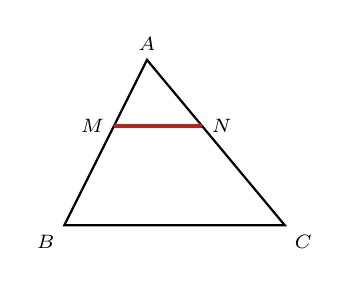
\begin{tikzpicture}[scale=0.7,font=\scriptsize]
\coordinate (A) at (0,3); \coordinate (B) at (-1.5,0); \coordinate (C) at (2.5,0);
\coordinate (M) at ($(A)!0.4!(B)$); \coordinate (N) at ($(A)!0.4!(C)$);
\draw[thick] (A)--(B)--(C)--cycle; \draw[cThm,very thick] (M)--(N);
\node[above] at (A){$A$}; \node[below left] at (B){$B$}; \node[below right] at (C){$C$};
\node[left] at (M){$M$}; \node[right] at (N){$N$};
\end{tikzpicture}\end{LTR}\par}{50 د}{نرسم شكل طالس.}
\Row{}{%
\Lab{cThm}{النسب المثلثية}\ في مثلث قائم: $\cos=\dfrac{\text{المجاور}}{\text{الوتر}}$ ، $\sin=\dfrac{\text{المقابل}}{\text{الوتر}}$ ، $\tan=\dfrac{\text{المقابل}}{\text{المجاور}}$.\par\Lab{cThm!80!black}{حذار}\ نطبق فيثاغورس في المثلث القائم فقط ، والوتر هو أطول ضلع.}{}{}
\Row{التقويم}{%
\Lab{cEx}{تطبيق}\par\Num{1} هل المثلث الذي أطواله $5$ ، $12$ ، $13$ قائم؟ \Num{2} $AM=2$ ، $AB=6$ ، $AC=9$ ، $BC=7{,}5$ و $(MN)\parallel(BC)$: احسب $AN$ و $MN$.\par\textbf{الحل:} \Num{1} $25+144=169$: نعم ؛ \Num{2} $AN=3$ و $MN=2{,}5$.\par\textbf{واجب منزلي:} تمارين من الكتاب المدرسي.\par\smallskip\textbf{ملاحظات حول سير الحصة:} \dotfill}{25 د}{تقويم فردي.}
\end{Sayr}
\newpage
\ModhHead{39}{1 ج م ع ت}{هندسة}{الهندسة المستوية}{02 سا}{الزوايا والدائرة}%
{\begin{itemize}\item الزوايا في مثلث.\item الدائرة.\end{itemize}}%
{\begin{itemize}\item معرفة العلاقة بين الزاوية المحيطية والزاوية المركزية.\item استعمال الدائرة لإثبات أن مثلثاً قائم.\end{itemize}}%
{المنهاج ، الكتاب المدرسي ، مراجع ، أدوات الهندسة.}
\begin{Sayr}
\Row{مرحلة الانطلاق}{%
\textbf{التهيئة النفسية:} ارسم دائرة وقطراً $[AB]$ ونقطة $M$ منها. قس الزاوية $\widehat{AMB}$. ماذا تلاحظ؟}{10 د}{تجربة بالمنقلة.}
\Row{التشخيص والاكتشاف}{%
\Lab{cEx}{مناقشة نشاط 05 صفحة 210}\par\ck\ المثلثان $AOM$ و $BOM$ متقايسا الساقين ، ومنه $\widehat{AMB}=90^\circ$ كلما كان $[AB]$ قطراً.\par
\ck\ بقياس عدة نقط $M$ على نفس القوس: $\widehat{AMB}$ ثابتة وتساوي نصف الزاوية المركزية $\widehat{AOB}$.\par
}{35 د}{نقارن قياسات التلاميذ.}
\Row{بناء المعارف}{%
\Lab{cThm}{خاصية}\par\ck\ الزاوية المحيطية تساوي نصف الزاوية المركزية التي تحصر نفس القوس: $\widehat{AMB}=\dfrac12\widehat{AOB}$.\par
\ck\ زاويتان محيطيتان تحصران نفس القوس متقايستان.\par
\ck\ $ABC$ قائم في $A$ $\iff A$ تنتمي إلى الدائرة التي قطرها $[BC]$.\par
\par\smallskip\begin{LTR}\centering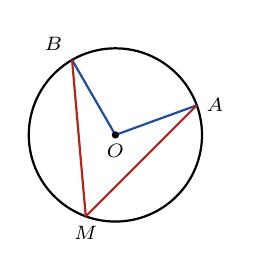
\begin{tikzpicture}[scale=1.1,font=\scriptsize]
\draw[thick] (0,0) circle (1);
\coordinate (O) at (0,0); \coordinate (A) at (20:1); \coordinate (B) at (120:1); \coordinate (M) at (250:1);
\draw[cDef,thick] (O)--(A) (O)--(B); \draw[cThm,thick] (M)--(A) (M)--(B);
\fill (O) circle (1.2pt) node[below]{$O$}; \node[right] at (A){$A$}; \node[above left] at (B){$B$}; \node[below] at (M){$M$};
\end{tikzpicture}\end{LTR}\par\Lab{cEx}{مثال}\ إذا كانت $\widehat{AOB}=100^\circ$ فإن $\widehat{AMB}=50^\circ$.\par}{50 د}{نرسم الشكل على السبورة.}
\Row{}{%
\Lab{cThm!80!black}{حذار}\ يجب أن تحصر الزاويتان نفس القوس.}{}{}
\Row{التقويم}{%
\Lab{cEx}{تطبيق}\par\Num{1} $[AB]$ قطر و $M$ من الدائرة: ما قيس $\widehat{AMB}$ ؟ \Num{2} $\widehat{AOB}=140^\circ$: احسب الزاوية المحيطية.\par\textbf{الحل:} \Num{1} $90^\circ$ ؛ \Num{2} $70^\circ$.\par\textbf{واجب منزلي:} تمارين من الكتاب المدرسي.\par\smallskip\textbf{ملاحظات حول سير الحصة:} \dotfill}{25 د}{تقويم فردي.}
\end{Sayr}
\newpage
\ModhHead{40}{1 ج م ع ت}{هندسة}{الهندسة المستوية}{02 سا}{المثلثات المتقايسة والمثلثات المتشابهة}%
{\begin{itemize}\item مبرهنة طالس.\item الزوايا.\end{itemize}}%
{\begin{itemize}\item التعرّف على مثلثين متقايسين ومثلثين متشابهين.\item استعمال حالات التقايس والتشابه في البرهان والحساب.\end{itemize}}%
{المنهاج ، الكتاب المدرسي ، مراجع ، أدوات الهندسة.}
\begin{Sayr}
\Row{مرحلة الانطلاق}{%
\textbf{التهيئة النفسية:} صورتان لنفس المبنى بمقاسين مختلفين: ما الذي يبقى ثابتاً؟}{10 د}{صورة من الحياة اليومية.}
\Row{التشخيص والاكتشاف}{%
\Lab{cEx}{مناقشة النشاطين 06 صفحة 210 و 07 صفحة 211}\par\ck\ بإنشاء مثلثات بمعطيات الجدول نلاحظ أن ثلاثة أضلاع ، أو ضلعين والزاوية المحصورة ، أو ضلعاً وزاويتين تحدد المثلث: \textbf{حالات التقايس}.\par
\ck\ مثلثان لهما نفس الزوايا: أضلاعهما متناسبة: \textbf{مثلثان متشابهان}.\par
}{35 د}{إنشاءات بالمعطيات.}
\Row{بناء المعارف}{%
\Lab{cThm}{حالات التقايس}\ (ض ، ض ، ض) ؛ (ض ، ز ، ض) ؛ (ز ، ض ، ز).\par\Lab{cThm}{حالات التشابه}\ زاويتان متقايستان مثنى مثنى ؛ أو أضلاع متناسبة ؛ أو زاوية متقايسة وضلعاها متناسبان.\par}{50 د}{نلخص الحالات في جدول.}
\Row{}{%
\Lab{cThm}{خاصية}\ إذا كان مثلثان متشابهين بنسبة $k$ فإن مساحتيهما $S^{\prime}=k^2S$.\par\Lab{cEx}{مثال}\ $M\in[AB]$ ، $N\in[AC]$ و $(MN)\parallel(BC)$ ، $AM=2$ ، $AB=5$: $AMN$ و $ABC$ متشابهان بنسبة $\dfrac25$ ، وإذا كانت مساحة $ABC$ هي $50$ cm² فمساحة $AMN$ هي $\Big(\dfrac25\Big)^2\times50=8$ cm².\par}{}{}
\Row{}{%
\Lab{cThm!80!black}{حذار}\ نسبة المساحات $k^2$ وليس $k$.}{}{}
\Row{التقويم}{%
\Lab{cEx}{تطبيق}\par $ABCD$ متوازي أضلاع مركزه $O$. بيّن أن المثلثين $OAB$ و $OCD$ متقايسان واستنتج $AB=CD$.\par\textbf{الحل:} $OA=OC$ ، $OB=OD$ و $\widehat{AOB}=\widehat{COD}$ (متقابلتان بالرأس): الحالة (ض ، ز ، ض).\par\textbf{واجب منزلي:} تمارين من الكتاب المدرسي.\par\smallskip\textbf{ملاحظات حول سير الحصة:} \dotfill}{25 د}{تقويم فردي.}
\end{Sayr}
\newpage
\ModhHead{41}{1 ج م ع ت}{هندسة}{الهندسة المستوية}{02 سا}{التحويلات النقطية: التناظر ، الانسحاب ، الدوران}%
{\begin{itemize}\item التناظر المحوري والمركزي ، الانسحاب.\end{itemize}}%
{\begin{itemize}\item معرفة التحويلات النقطية وخواصها.\item إنشاء صورة شكل بتحويل.\end{itemize}}%
{المنهاج ، الكتاب المدرسي ، مراجع ، أدوات الهندسة.}
\begin{Sayr}
\Row{مرحلة الانطلاق}{%
\textbf{التهيئة النفسية:} زخارف جزائرية تقليدية: ما التحويلات التي تكرر الشكل؟}{10 د}{ربط بالتراث.}
\Row{التشخيص والاكتشاف}{%
\Lab{cEx}{مناقشة نشاط 08 صفحة 211}\par\ck\ بالورق الشفاف: صورة مثلث بانسحاب أو تناظر أو دوران مثلث يقايسه.\par
\ck\ التناظر المحوري يعكس اتجاه الدوران ، والانسحاب والتناظر المركزي والدوران تحافظ عليه.\par
}{35 د}{عمل بالورق الشفاف.}
\Row{بناء المعارف}{%
\Lab{cDef}{تعريف}\par\ck\ \textbf{الانسحاب} الذي شعاعه $\vec u$: $\overrightarrow{MM^{\prime}}=\vec u$.\par
\ck\ \textbf{التناظر المركزي} بالنسبة إلى $O$: $O$ منتصف $[MM^{\prime}]$.\par
\ck\ \textbf{التناظر المحوري} بالنسبة إلى $(\Delta)$: $(\Delta)$ محور $[MM^{\prime}]$.\par
\ck\ \textbf{الدوران} الذي مركزه $O$ وزاويته $\theta$: $OM^{\prime}=OM$ و $\widehat{MOM^{\prime}}=\theta$ في الاتجاه المحدد.\par
\Lab{cThm}{خاصية}\ هذه التحويلات تحافظ على الأطوال والزوايا والمساحات والاستقامية والتوازي: صورة شكل شكل يقايسه.\par}{50 د}{جدول خواص التحويلات.}
\Row{}{%
\Lab{cEx}{مثال}\ صورة دائرة مركزها $O$ ونصف قطرها $3$ بانسحاب هي دائرة نصف قطرها $3$ ومركزها صورة $O$.\par\Lab{cThm!80!black}{حذار}\ التناظر المركزي دوران زاويته $180^\circ$.}{}{}
\Row{التقويم}{%
\Lab{cEx}{تطبيق}\par $ABCD$ مربع مركزه $O$. ما صورة المربع بالدوران الذي مركزه $O$ وزاويته $90^\circ$ ؟\par\textbf{الحل:} المربع نفسه: $A\mapsto B$ ، $B\mapsto C$ ، $C\mapsto D$ ، $D\mapsto A$ (في الاتجاه المناسب).\par\textbf{واجب منزلي:} تمارين من الكتاب المدرسي.\par\smallskip\textbf{ملاحظات حول سير الحصة:} \dotfill}{25 د}{تقويم فردي.}
\end{Sayr}
\newpage
\ModhHead{42}{1 ج م ع ت}{هندسة}{الهندسة المستوية}{02 سا}{حل مسائل: محال هندسية وإنشاءات}%
{\begin{itemize}\item المستقيمات الخاصة ، الدائرة ، التحويلات.\end{itemize}}%
{\begin{itemize}\item تعيين محل هندسي.\item إنجاز إنشاءات هندسية وتبريرها.\end{itemize}}%
{المنهاج ، الكتاب المدرسي ، مراجع ، أدوات الهندسة.}
\begin{Sayr}
\Row{مرحلة الانطلاق}{%
\textbf{التهيئة النفسية:} أين تقع كل النقط التي تبعد $3$ cm عن نقطة $O$ ؟ وكل النقط التي تبعد بنفس المسافة عن $A$ و $B$ ؟}{10 د}{سؤال يقود إلى المحل الهندسي.}
\Row{التشخيص والاكتشاف}{%
\Lab{cEx}{وضعية مقترحة}\par نريد بناء بئر على طريق مستقيم $(d)$ بحيث يبعد بنفس المسافة عن منزلين $A$ و $B$. أين نضعه؟\par\ck\ النقط المتساوية البعد عن $A$ و $B$ هي محور $[AB]$.\par
\ck\ البئر هو نقطة تقاطع محور $[AB]$ مع $(d)$ (إن وُجدت).\par
}{35 د}{عمل في مجموعات على الخريطة.}
\Row{بناء المعارف}{%
\Lab{cDef}{تعريف}\ \textbf{المحل الهندسي} مجموعة النقط التي تحقق خاصية معينة.\par\Lab{cThm}{محال مألوفة}\par\ck\ النقط التي تبعد $r$ عن $O$: الدائرة التي مركزها $O$ ونصف قطرها $r$.\par
\ck\ النقط المتساوية البعد عن $A$ و $B$: محور $[AB]$.\par
\ck\ النقط المتساوية البعد عن ضلعي زاوية: منصفها.\par
\ck\ النقط $M$ حيث $\widehat{AMB}=90^\circ$: الدائرة التي قطرها $[AB]$ (باستثناء $A$ و $B$).\par
}{50 د}{ملخص المحال المألوفة.}
\Row{}{%
\Lab{cMeth}{طريقة}\ نخمّن بالرسم ، ثم نبرهن بالخواص ، ثم ننشئ ونبرر الإنشاء.\par\Lab{cThm!80!black}{حذار}\ نتأكد من الاحتواءين: كل نقطة من المحل تحقق الخاصية ، وكل نقطة تحققها تنتمي إليه.}{}{}
\Row{التقويم}{%
\Lab{cEx}{تطبيق}\par أنشئ مثلثاً $ABC$ حيث $AB=5$ ، $BC=4$ ، $AC=3$ ، ثم أنشئ دائرته المحيطة. ما طبيعة المثلث؟ أين يقع مركز الدائرة؟\par\textbf{الحل:} $9+16=25$: قائم في $C$ ، ومركز الدائرة منتصف $[AB]$.\par\textbf{واجب منزلي:} تمارين حوصلة المحور من الكتاب المدرسي.\par\smallskip\textbf{ملاحظات حول سير الحصة:} \dotfill}{25 د}{نهاية المحور: فرض أو تمارين حوصلة.}
\end{Sayr}
\end{document}
